\section{Integration Architecture}
\label{sec:architecture}
As discussed in Section \ref{sec:related}, this paper focuses on the proposed testbed as an integral part of the RAMPART cyber agent training workflow. Although we confine our discussion here to the OT networks, it is important to note that the integration architecture and the base images used are inherited from the RAMPART network topology or the $CAGE-2$ topology as shown in Figure \ref{fig:Enterprise_Network}. Moving forward, the larger network that the OT network is integrated into will be referred to as the enterprise network.

In this testbed, we deploy two specific OT use cases, a Power Grid and a Chemical Plant. 
% \begin{itemize}
%     \item \textbf{Power Grid} - hosted as a single host-only-network within the enterprise network,
%     \item \textbf{Chemical Plant} - hosted as a subnet consisting of three hosts within the enterprise network.
% \end{itemize}
Using the support from different software modules we replicate the real-world dynamics of a power grid and a chemical plant on OpenStack hosts, which makes it a realistic testbed for testing and evaluating cyber agents for OT networks. OpenStack is an open-source cloud computing platform that provides a set of software tools for building and managing cloud computing environments.
% It enables researchers and businesses to deploy virtual servers and other resources such as storage and networking services, enabling them to create scalable and flexible cloud infrastructure. OpenStack is designed to facilitate the widespread adoption of cloud services by being hardware-agnostic and providing a high degree of control over the environment. It provides a user friendly interface to design network topologies and host devices connected to them along with the required peripherals.
As the enterprise network with the \textit{CAGE-2} \cite{kiely2023autonomousagentscyberdefence} topology is built on OpenStack, we conformed to the \textit{CAGE-2} integration rules for building the OT network.
\subsection{Power Grid}
This use case replicates a real-world scenario of a smart grid consisting of three substations and a power house as shown in the Figure \ref{fig:powergrid}. This example underlines the importance of securing OT networks in smart grids. The working of the power grid emulator is governed by three important components; all installed on a single host machine connected to the enterprise network.
\begin{figure}[!ht]
    \centering
    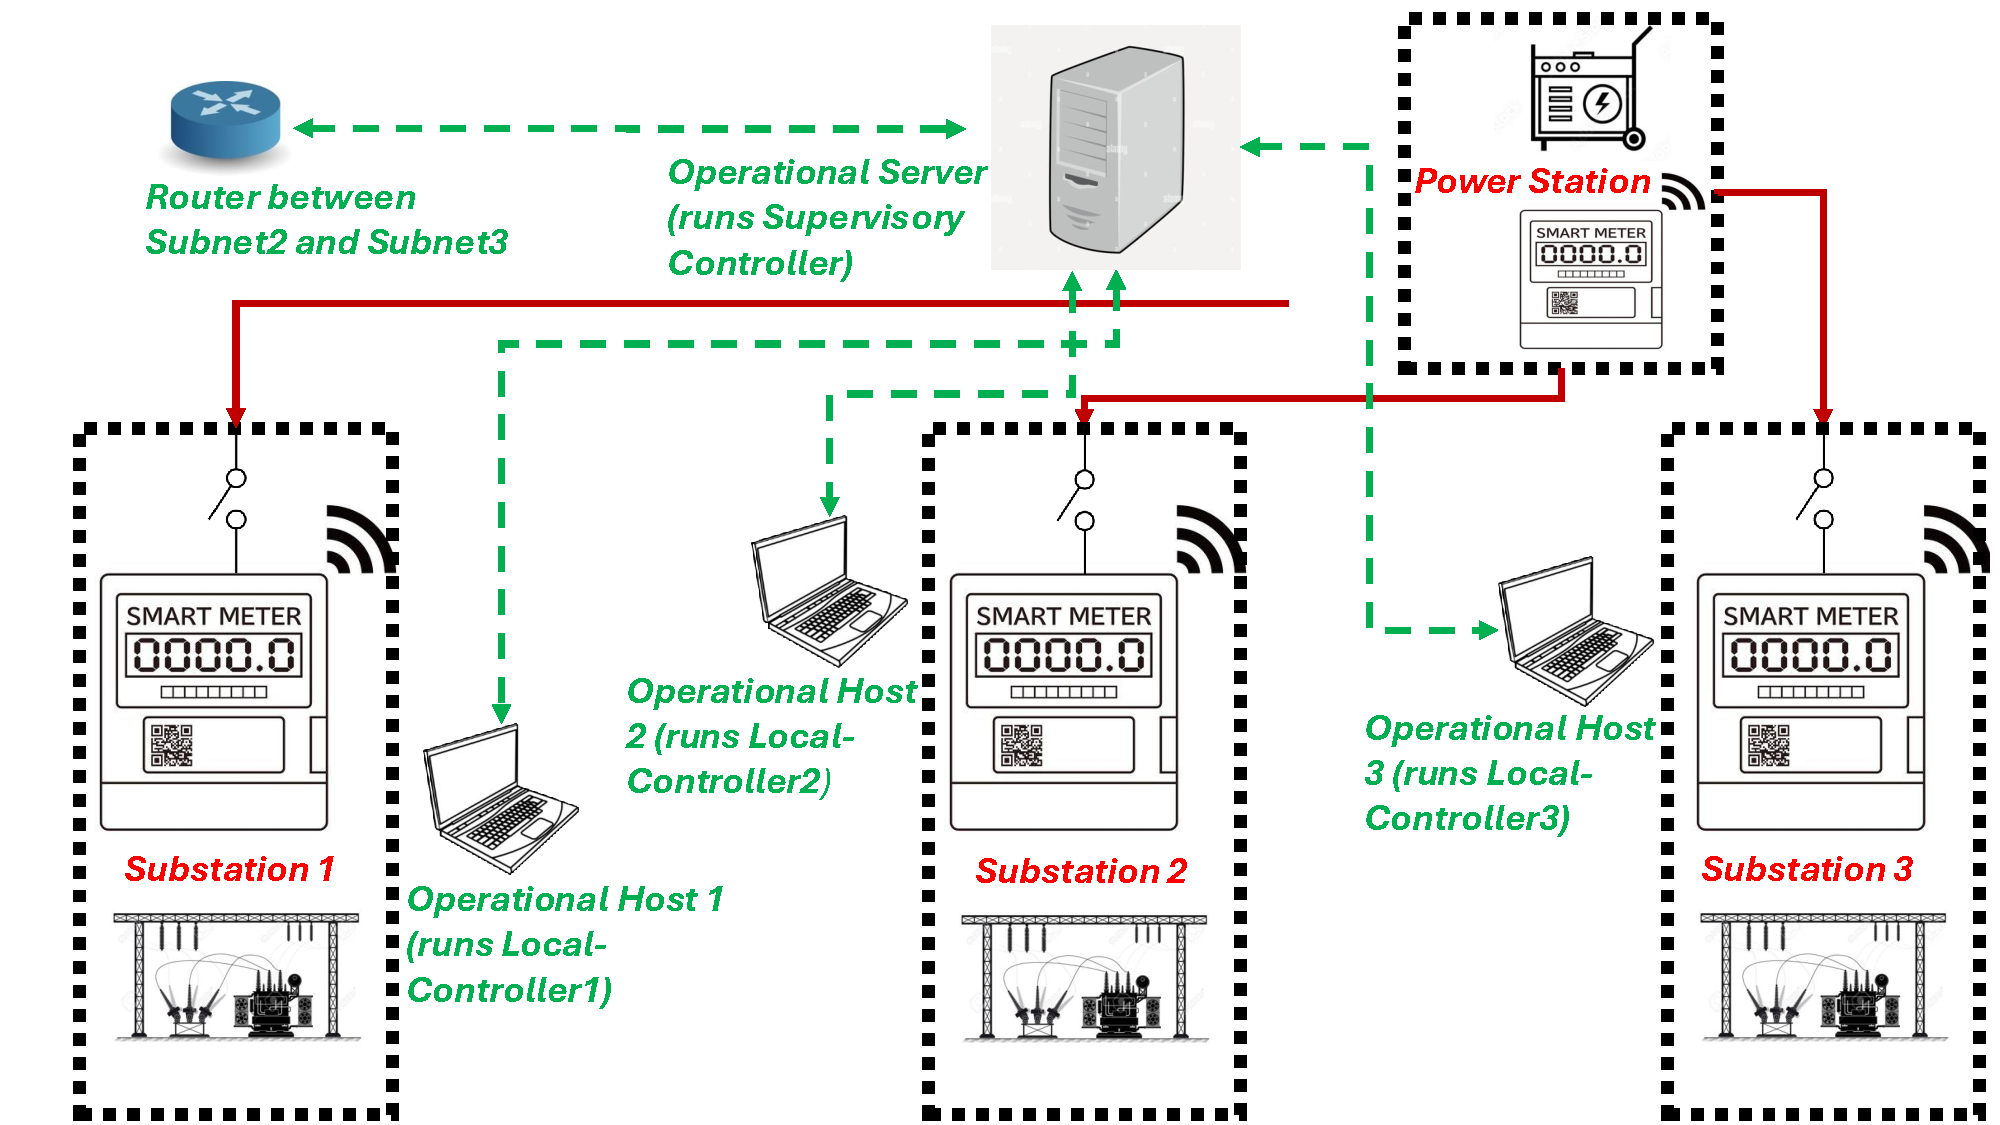
\includegraphics[width=\linewidth, trim=0.25cm 0.5cm 0cm 0cm]{Figures/powergridotnw_new.pdf}
    \caption{Block diagram depicting the use of OT networks in Smart Grids and the underlying hardware-software integration. The red line represents the Power grid operations (GridLAB-D emulations) and the green corresponds to the OT networks (Mininet emulation).}
    \label{fig:powergrid}
% \vspace{-0.6cm}
\end{figure}
\subsubsection{GridLAB-D} It is an advanced power distribution system simulation and analysis tool, aiding designers, operators, and utilities in optimizing energy technologies \cite{chassin2014gridlab}. Developed by the U.S. Department of Energy at Pacific Northwest National Laboratory, it features cutting-edge modeling techniques and distribution automation models using a variety of modules designed for a variety of use-cases. We use this software as the simulation platform replicating a real-world power grid system. In the real-world micro-grid and smart-grid scenarios, the regulators and controllers used to maintain the desired power and performance metrics rely on the OT network for sensing and actuation. We recreate this behavior using GridLAB-D in the server mode. The server mode of GridLAB-D (v4.3) enables the OT network to communicate with the grid using standard TCP/IP protocols.
% We use the GridLAB-D v4.3 for our experiments.
Here we highlight some of the key components of GridLAB-D used in this testbed:
\begin{itemize}
    \item \textit{Generator} object hosts a variety of power sources with control including simple solar models, wind turbine models, and battery control models. 
    % This module helps create an open environment for distributed generation, where users can create their own models, including control algorithms.
    \item \textit{Meters} are general purpose energy and power meters. These are useful for time-varying simulations with recorder objects attached for data collection.
    % GridLAB-D's normal output methods (.xml, .txt) will only record the final time-step of a system, so for time varying systems a recorder and meter are needed to track power and energy, as well as voltage and current.
    \item \textit{Recorder} provides the ability to collect a recording of one or more properties of an object with user-defined sampling interval, triggers, and other properties.
    \item Switch object serves as the simple electrical disconnect device. This object acts as an actuator in the testbed.
    \item \textit{Overhead lines}  provides configurable (resistance, length, material etc.) object as connecting components.
    \item \textit{Load} is a configurable object to represent a generic power sink with phases, voltage, and current parameters.
    % \item Zip-Load : The ZIPload model is designed to provide a means to access the Residential class at a fundamental level and from a power engineer perspective. Users can design and connect the ZIPload to environment variables, that changes the power consumption of the load based on the weather data that gives it more realistic sim environment. 
\end{itemize}

\subsubsection{Mininet} It allows emulating simplified, scaled-down versions of real-world computer networks, often used for educational or experimental purposes \cite{10.1145/1868447.1868466}. It enables users to emulate network topologies, test network protocols, and study network behavior in a controlled environment, facilitating learning and research in networking concepts. In our setup, a single Mininet instance hosts the OT network, comprising four nodes. One node runs the supervisory controller (\textit{SC}) and the other three run the local controllers (\textit{LCs}). These controllers communicate with the \textit{GridLAB-D} server to monitor and report relevant system metrics.

% \vspace{-0.1cm}

\subsubsection{Two-Level Controllers} As shown in the Figure \ref{fig:powergrid}, the OT network consists of one Operational Server (OS) running the \textit{SC} and three operational hosts (OH) running the \textit{LCs} connected through a router. In the current setup, all nodes in the OT network are homogeneous, with their responsibilities and capabilities determined by the controllers running on them. These controllers play a crucial role in sensing key metrics of the grid and actuating components within the GridLAB-D simulator. Some of the key monitored parameters include three-phase power measurements, substation loads, switch statuses, and triplex meter readings.

The \textit{SC} is responsible for distributing power efficiently while preventing generator overload, based on the requirements and priority levels received from the \textit{LCs}. It continuously monitors the total power consumption across the three substation loads and generators, ensuring balanced distribution. 
Additionally, the \textit{SC} transmits regulatory information to the \textit{LCs}, enabling them to make informed decisions for localized power management.

The \textit{LCs} periodically collect measurements from GridLAB-D within their assigned scope. Every 5 seconds, they transmit data on future power demand and substation priority levels to the \textit{SC}. Upon receiving regulatory instructions from the \textit{SC}, the \textit{LCs} adjust the power distribution to ensure efficient grid operation.
% \end{itemize}
% The schematic of the power grid integrated with its corresponding network is as shown in the Figure \ref{fig:powergrid}.


Figure \ref{fig:powergrid} shows the schematic of the smart grid OT network consisting of a power grid simulator and the corresponding network.
% The power grid is simulated using GridLAB-D. It replicates the working of a power grid given consisting of a generator and three substations connected using overhead lines and switches. 
The power generator is designed to generate power at a constant voltage and deliver it to the substation through the overhead lines. The substations consist of loads designed to include utilities in the form of loads. These loads can be disconnected from the grid at any time with the help of the switch present at the substations. In the normal mode, the power station delivers the power based on the substation demands and priority levels at a constant voltage. 

In a Smart Grid, the \textit{LCs} at each substation calculate the power demand over predefined time intervals. Additionally, they determine the priority levels of these demands based on the types of loads connected to the substation. While various algorithms can be used to assign priorities, this testbed employs a random number generator to set priority levels for each load. The \textit{LCs} communicate the demand and priority data to the \textit{SC} via the OT network using the TCP/IP protocol. Upon receiving this information, the \textit{SC} re-calculate the power allocation across substations, ensuring that available power is distributed according to priority rankings. If the total requested power exceeds the power station’s capacity, substations with the lowest priority rankings experience a power shortage. If the shortage is severe enough -- meeting or exceeding the demand of lower-priority substations -- some or all of these substations enter islanding mode. 
% In this mode, substations are disconnected from the grid for the remainder of the current interval by opening their corresponding switches. 
The operator can monitor the requests of each of the controllers and the corresponding power allocation through the visualizer present locally at the node. 

% The primary controller can visualize the demand and usage using the visualization tool present locally as shown in the Figure \ref{fig:Visualizer}.
% \begin{figure}[H]
%     \centering
%     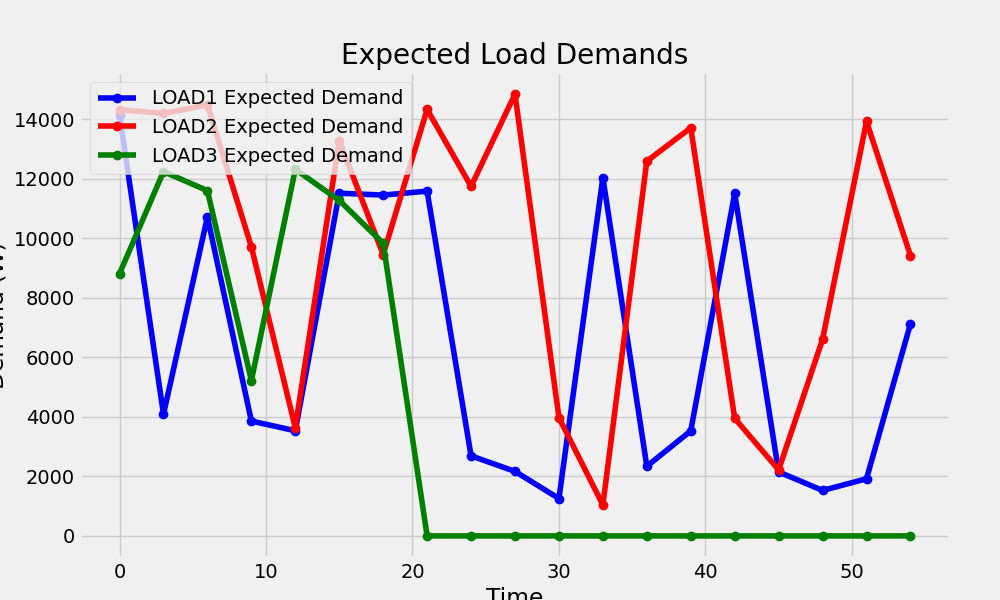
\includegraphics[width=\linewidth]{Figures/expected_load_demands_lc3_dos.png}
%     % \todo{Wrong figure.}
%     \caption{Live Visualization of the power generated and the power consumed by each load.}
%     \label{fig:Visualizer}
% \end{figure}


% \begin{figure}
%     \centering
%     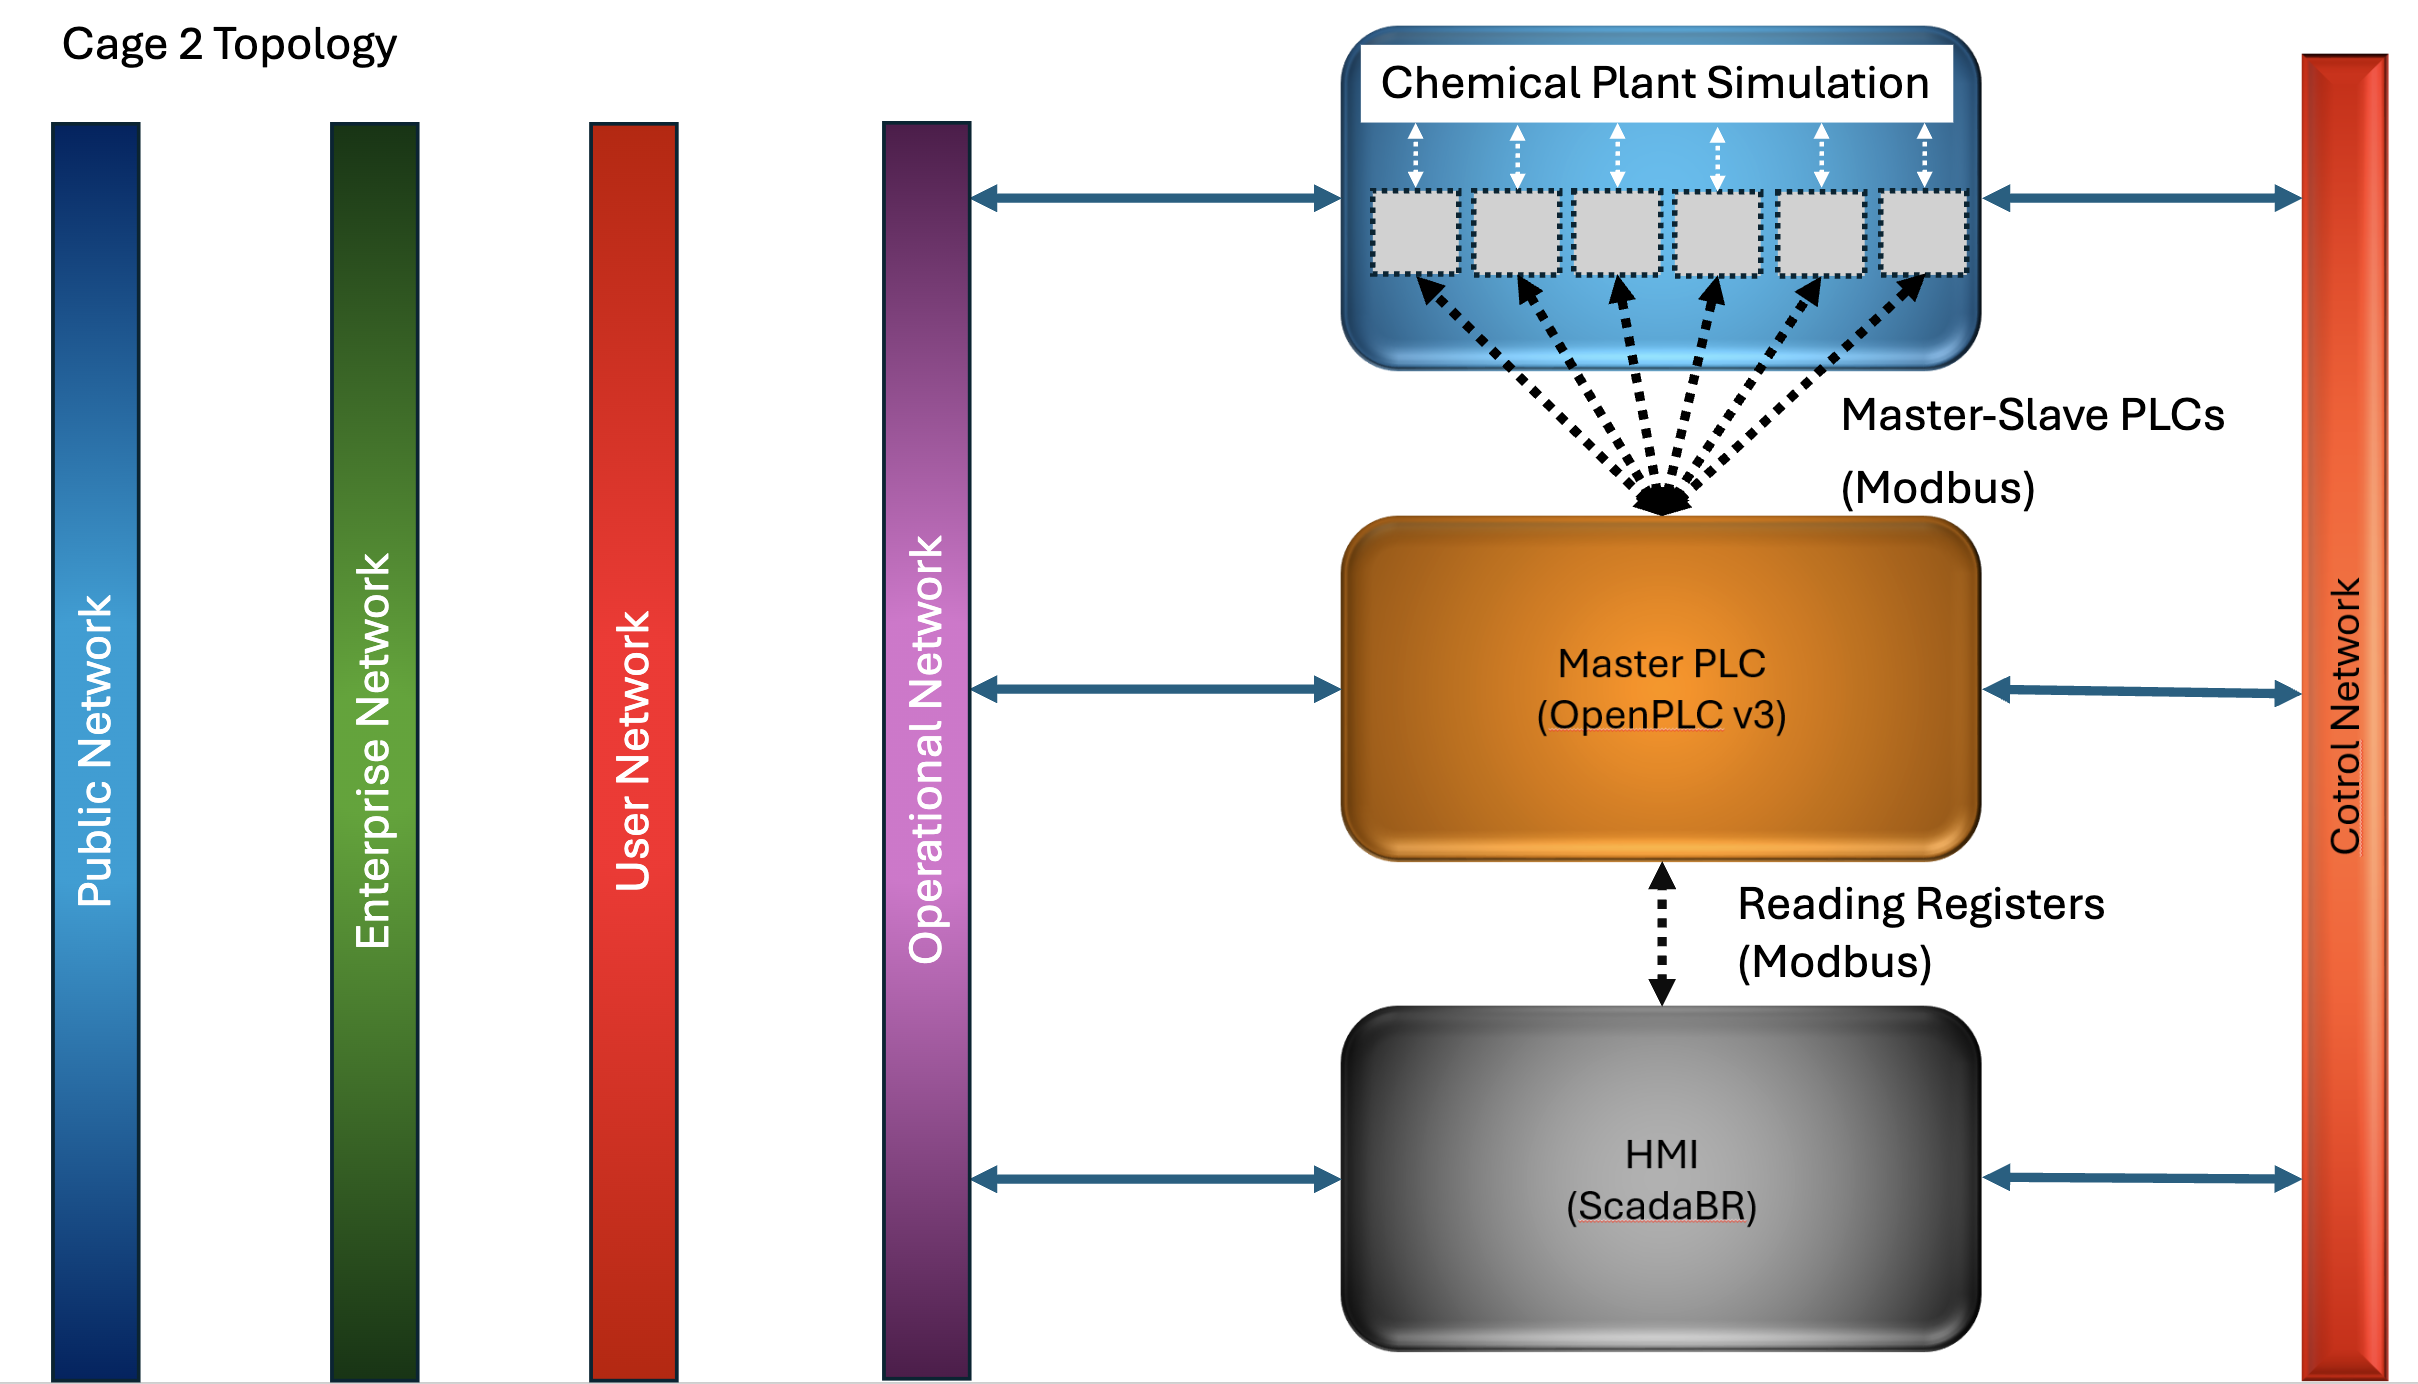
\includegraphics[width=\linewidth]{Figures/ChemicalPlantNW.png}
%     \caption{A schematic of the Chemical plant OT network depicting the }
%     \label{fig:Chemical Plant}
% \end{figure}

% \vspace{-0.2cm}
\subsection{Chemical Plant}
The Chemical Plant Workflow is the adaptation of the testbed used for the experiments related to Industrial Control Systems (ICS) by David et al. \cite{formby2018lowering}. The main components of this OT workflow are:
\subsubsection{Graphical Realism Framework For ICS (GRFICS):} We use GRFICS ~\cite{formby2018lowering} for developing a use-case by hosting its different components on the openstack host machines.
The GRFICS was designed as a modular system 
for customization and scalability, using standard ICS network protocols to connect elements like Human Machine Interface (HMI), Programmable Logic Control (PLC), and Input/Output (I/O) modules, and permits the interchanging of these components with actual ICS devices. It integrates physical process simulation with 3D visualization and the I/O module layer through a user-friendly JSON-based network API.
    % The simulation backend efficiently calculates the current state of a simplified version of an industrial chemical process-control problem, involving complex exothermic reactions and multiple variables to monitor and adjust for safety and efficiency.
    The simulation backend computes the current state of a simplified industrial chemical process, incorporating complex exothermic reactions. These reactions involve multiple critical variables that must be continuously monitored and adjusted to ensure safety and operational efficiency. Figure \ref{fig:GRFICS} presents a simplified model of the underlying process, reduced to a two-phase chemical reactor/separator \cite{downs1993plant}. With fewer control 
    \begin{figure}[htb]
    \centering
    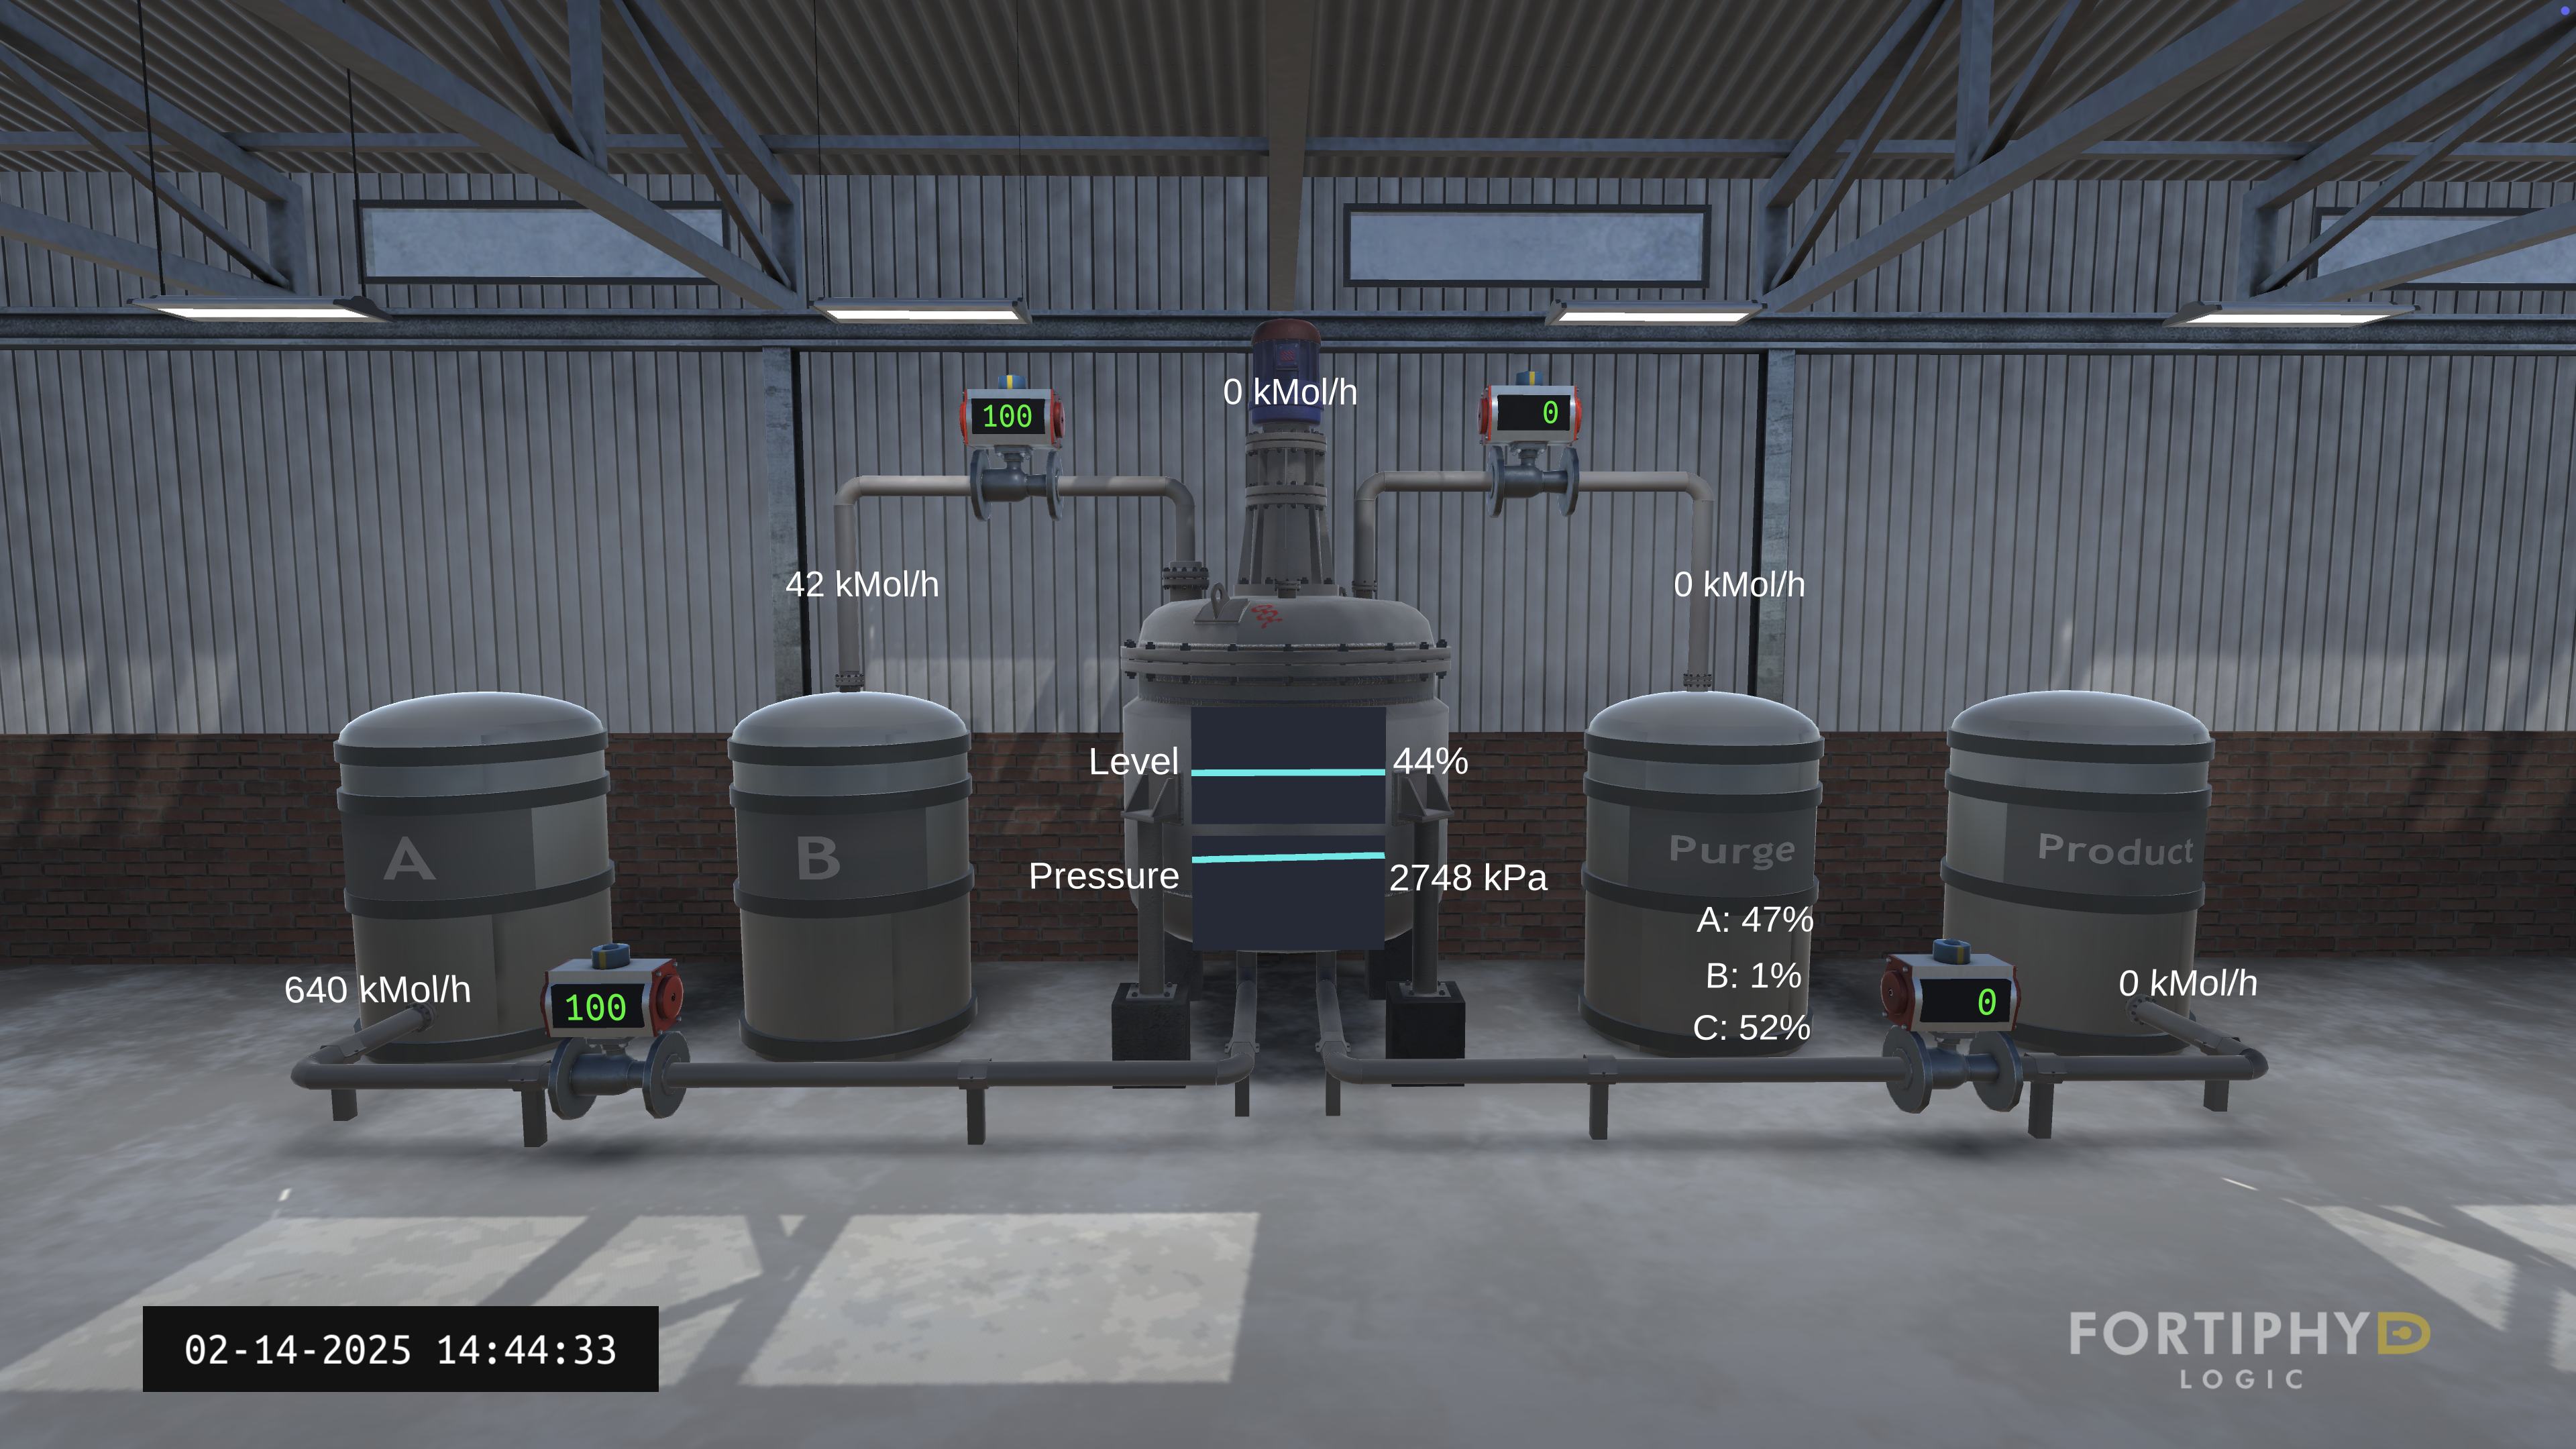
\includegraphics[keepaspectratio, width=0.6\linewidth]{Figures/Stage_1.png}
    \caption{GRFICS visualizer.}
    \label{fig:GRFICS}
\end{figure}
      valves and limited output measurements, this use case focuses on maintaining safe reactor pressure, optimizing chemical reaction efficiency, and minimizing waste. The controlled variables are two feed valves corresponding to the reactants (A and B), and the two output valves corresponding to the product (C) and purge tanks, respectively. The regulation of these valves at user-defined setpoints ensures system stability and safety, which is continuously monitored through sensor observations of pressure, liquid levels, and purge compositions. A Proportional-Derivative (PD) controller regulates the valve positions at user-defined setpoints through a master-slave Programmable Logic Controller (PLC).
    This emulation is hosted on a dedicated host machine within the OT network, labeled as the chemical plant in Figure \ref{fig:Chemical Plant}. The shaded squares within the chemical plant represent PLC slaves, which transmit sensor measurements to the master PLC for decision-making.

    \begin{figure}[!ht]
%     \vspace{-0.4cm}
\begin{tikzpicture}
    \node[draw, rectangle, rounded corners, minimum width=3cm, minimum height=1.5cm, fill=blue!30, xshift=0cm] (rect1) {};
    \node[label={[yshift=0.075cm]north:Chemical Plant}] at (rect1.center) {};
    \foreach \x [count=\xi] in {1,...,6} {
        \coordinate (square-\xi) at ([xshift=-0.25cm + \x*0.45cm, yshift=0.5cm] rect1.south west);
        \draw (square-\xi) rectangle ++(0.35cm,0.35cm);
    }
    \foreach \x in {1,...,6} {
        \draw[fill=gray] ([xshift=-0.25cm + \x*0.45cm, yshift=0.5cm] rect1.south west) rectangle ++(0.35cm,0.35cm);
    }

    \node[draw, rectangle, rounded corners, minimum width=3cm, minimum height=1.5cm, fill=red!30, below=1cm of rect1] (rect2) {Master PLC};
    \node[draw, rectangle, rounded corners, minimum width=3cm, minimum height=1.5cm, fill=gray!30, below=1cm of rect2] (rect3) {Operator};
    \coordinate (top point) at ([xshift=4cm,yshift=0cm] rect1.north);
    \coordinate (bottom point) at ([xshift=4cm,yshift=0cm] rect3.south);
    % Adjusted distances to create gaps
\node[draw, rectangle, minimum width=6.5cm, minimum height=0.2cm, fill=cyan!60!white, rotate=270, right=-1.8cm of rect1.east] (controlrect) at ($(top point)!0!(bottom point)$) {{Control Network}};
\node[draw, rectangle, minimum width=6.5cm, minimum height=0.2cm, fill=violet!60!white, rotate=90, left=9.5cm of rect1.west] (publicrect) at ($(top point)!0!(bottom point)$) {{Internet}};
\node[draw, rectangle, minimum width=6.5cm, minimum height=0.2cm, fill=green!60!white, rotate=90, left=8.5cm of rect1.west] (enterrect) at ($(top point)!0!(bottom point)$) {{Enterprise Subnet}};
\node[draw, rectangle, minimum width=6.5cm, minimum height=0.2cm, fill=red!50!yellow, rotate=90, left=7.5cm of rect1.west] (userrect) at ($(top point)!0!(bottom point)$) {{User Subnet}};
\node[draw, rectangle, minimum width=6.5cm, minimum height=0.2cm, fill=black!50!white, rotate=90, left=6.5cm of rect1.west] (optrect) at ($(top point)!0!(bottom point)$) {{Operational Subnet}};

% The rest of the Ti*k*Z code remains the same...
    \foreach \x in {1,...,6} {
        \draw[Latex-Latex] (rect2.north) -- ($(square-\x.south)+(0.175,0cm)$);
    }
            \draw[thick, -Latex, blue] ([xshift=0.25cm, yshift=0.25cm]square-1) to[bend left] ([xshift=-0.5cm, yshift=0.7cm]square-1) node[anchor=south west,xshift=-0.4cm, blue] {PLC Slave};
    \draw[{Latex}-{Latex}] (publicrect.south) -- (enterrect.north);
    \draw[{Latex}-{Latex}] (enterrect.south) -- (userrect.north);
    \draw[{Latex}-{Latex}] (userrect.south) -- (optrect.north);
            
    \draw[thick, {Latex[length=2mm]}-{Latex[length=2mm]}] (rect1.east) -- ($(controlrect.south)+(0cm,2.5cm)$);
    \draw[thick, {Latex[length=2mm]}-{Latex[length=2mm]}] (rect2.east) -- ($(controlrect.south)+(0cm,0cm)$);
    \draw[thick, {Latex[length=2mm]}-{Latex[length=2mm]}] (rect3.east) -- ($(controlrect.south)+(0cm,-2.5cm)$);
    \draw[thick, {Latex[length=2mm]}-{Latex[length=2mm]}] (rect2.south) -- (rect3.north);
    \draw[thick, {Latex[length=2mm]}-{Latex[length=2mm]}] (rect1.west) -- ($(optrect.south)+(0cm,2.5cm)$);
    \draw[thick, {Latex[length=2mm]}-{Latex[length=2mm]}] (rect2.west) -- ($(optrect.south)+(0cm,0cm)$);
    \draw[thick, {Latex[length=2mm]}-{Latex[length=2mm]}] (rect3.west) -- ($(optrect.south)+(0cm,-2.5cm)$);
    
\end{tikzpicture}
% \vspace{-0.3cm}
    \caption{Chemical Plant workflow in Openstack.}
    \label{fig:Chemical Plant}
%     \vspace{-0.5cm}
\end{figure}
    \subsubsection{OpenPLC} It is an open-source PLC designed for ease of use, offering a cost-effective industrial automation solution suitable for both research and practical applications \cite{6970342}. It is compatible with a wide range of operating systems and, like traditional industrial PLCs, supports both discrete and continuous input interfaces through discrete input registers and coils, respectively. OpenPLC provides users with access to a limited set of registers, categorized as input, read and write registers, each named according to its specific function. The values stored in these registers can be utilized for informed decision-making, with controller logic programmed in standard PLC languages such as Structured Text (ST) and Ladder Diagram (LD). The PLC’s capacity can be expanded by connecting supported Modbus TCP devices, allowing additional slave PLCs to interface with the master PLC. Using Modbus, slave devices can read from and write to the master PLC’s registers via a standardized addressing system. This capability enables Modbus slaves to report sensor values to the master PLC by writing to its input registers and to execute controller decisions by reading from its holding registers. Modbus TCP utilizes TCP/IP for data exchange between devices such as PLCs and sensors, offering improved performance, scalability, and seamless integration with existing network infrastructures. Its reliability, even in harsh industrial environments, has made it a preferred choice for industrial communication.
    However, in Modbus TCP, packets are transmitted unencrypted to prioritize speed and efficiency, which makes the protocol susceptible to data falsification attacks and other cyber-threats, thereby limiting its use to industrial applications.
%    However, Modbus TCP is vulnerable to security risks, limiting its use to industrial applications. As packets are transmitted unencrypted, prioritizing speed and efficiency, the protocol is susceptible to data falsification attacks and other cyber threats. 
    
    \subsubsection{OpenPLC Client} It is a Python API that generates Modbus TCP API calls to interact with OpenPLC. Through its client interface, users can read and write the OpenPLC coils and registers. In our setup, the OpenPLC client runs on the operator node, where it reads and writes the OpenPLC registers and coils thereby
    % Additionally, the client can address both master and slave PLC devices, capturing and storing reported measurements in a database on the operator host for further analysis. 
    % By using the OpenPLC client for data monitoring and control, we
    bypassing the use of a dedicated Supervisory Control and Data Acquisition (SCADA) software like ScadaBR \cite{6938840}.
    
    












